\documentclass[]{article}
\usepackage{lmodern}
\usepackage{amssymb,amsmath}
\usepackage{ifxetex,ifluatex}
\usepackage{fixltx2e} % provides \textsubscript
\ifnum 0\ifxetex 1\fi\ifluatex 1\fi=0 % if pdftex
  \usepackage[T1]{fontenc}
  \usepackage[utf8]{inputenc}
\else % if luatex or xelatex
  \ifxetex
    \usepackage{mathspec}
  \else
    \usepackage{fontspec}
  \fi
  \defaultfontfeatures{Ligatures=TeX,Scale=MatchLowercase}
\fi
% use upquote if available, for straight quotes in verbatim environments
\IfFileExists{upquote.sty}{\usepackage{upquote}}{}
% use microtype if available
\IfFileExists{microtype.sty}{%
\usepackage{microtype}
\UseMicrotypeSet[protrusion]{basicmath} % disable protrusion for tt fonts
}{}
\usepackage[margin=1in]{geometry}
\usepackage{hyperref}
\hypersetup{unicode=true,
            pdfborder={0 0 0},
            breaklinks=true}
\urlstyle{same}  % don't use monospace font for urls
\usepackage{color}
\usepackage{fancyvrb}
\newcommand{\VerbBar}{|}
\newcommand{\VERB}{\Verb[commandchars=\\\{\}]}
\DefineVerbatimEnvironment{Highlighting}{Verbatim}{commandchars=\\\{\}}
% Add ',fontsize=\small' for more characters per line
\usepackage{framed}
\definecolor{shadecolor}{RGB}{248,248,248}
\newenvironment{Shaded}{\begin{snugshade}}{\end{snugshade}}
\newcommand{\AlertTok}[1]{\textcolor[rgb]{0.94,0.16,0.16}{#1}}
\newcommand{\AnnotationTok}[1]{\textcolor[rgb]{0.56,0.35,0.01}{\textbf{\textit{#1}}}}
\newcommand{\AttributeTok}[1]{\textcolor[rgb]{0.77,0.63,0.00}{#1}}
\newcommand{\BaseNTok}[1]{\textcolor[rgb]{0.00,0.00,0.81}{#1}}
\newcommand{\BuiltInTok}[1]{#1}
\newcommand{\CharTok}[1]{\textcolor[rgb]{0.31,0.60,0.02}{#1}}
\newcommand{\CommentTok}[1]{\textcolor[rgb]{0.56,0.35,0.01}{\textit{#1}}}
\newcommand{\CommentVarTok}[1]{\textcolor[rgb]{0.56,0.35,0.01}{\textbf{\textit{#1}}}}
\newcommand{\ConstantTok}[1]{\textcolor[rgb]{0.00,0.00,0.00}{#1}}
\newcommand{\ControlFlowTok}[1]{\textcolor[rgb]{0.13,0.29,0.53}{\textbf{#1}}}
\newcommand{\DataTypeTok}[1]{\textcolor[rgb]{0.13,0.29,0.53}{#1}}
\newcommand{\DecValTok}[1]{\textcolor[rgb]{0.00,0.00,0.81}{#1}}
\newcommand{\DocumentationTok}[1]{\textcolor[rgb]{0.56,0.35,0.01}{\textbf{\textit{#1}}}}
\newcommand{\ErrorTok}[1]{\textcolor[rgb]{0.64,0.00,0.00}{\textbf{#1}}}
\newcommand{\ExtensionTok}[1]{#1}
\newcommand{\FloatTok}[1]{\textcolor[rgb]{0.00,0.00,0.81}{#1}}
\newcommand{\FunctionTok}[1]{\textcolor[rgb]{0.00,0.00,0.00}{#1}}
\newcommand{\ImportTok}[1]{#1}
\newcommand{\InformationTok}[1]{\textcolor[rgb]{0.56,0.35,0.01}{\textbf{\textit{#1}}}}
\newcommand{\KeywordTok}[1]{\textcolor[rgb]{0.13,0.29,0.53}{\textbf{#1}}}
\newcommand{\NormalTok}[1]{#1}
\newcommand{\OperatorTok}[1]{\textcolor[rgb]{0.81,0.36,0.00}{\textbf{#1}}}
\newcommand{\OtherTok}[1]{\textcolor[rgb]{0.56,0.35,0.01}{#1}}
\newcommand{\PreprocessorTok}[1]{\textcolor[rgb]{0.56,0.35,0.01}{\textit{#1}}}
\newcommand{\RegionMarkerTok}[1]{#1}
\newcommand{\SpecialCharTok}[1]{\textcolor[rgb]{0.00,0.00,0.00}{#1}}
\newcommand{\SpecialStringTok}[1]{\textcolor[rgb]{0.31,0.60,0.02}{#1}}
\newcommand{\StringTok}[1]{\textcolor[rgb]{0.31,0.60,0.02}{#1}}
\newcommand{\VariableTok}[1]{\textcolor[rgb]{0.00,0.00,0.00}{#1}}
\newcommand{\VerbatimStringTok}[1]{\textcolor[rgb]{0.31,0.60,0.02}{#1}}
\newcommand{\WarningTok}[1]{\textcolor[rgb]{0.56,0.35,0.01}{\textbf{\textit{#1}}}}
\usepackage{graphicx,grffile}
\makeatletter
\def\maxwidth{\ifdim\Gin@nat@width>\linewidth\linewidth\else\Gin@nat@width\fi}
\def\maxheight{\ifdim\Gin@nat@height>\textheight\textheight\else\Gin@nat@height\fi}
\makeatother
% Scale images if necessary, so that they will not overflow the page
% margins by default, and it is still possible to overwrite the defaults
% using explicit options in \includegraphics[width, height, ...]{}
\setkeys{Gin}{width=\maxwidth,height=\maxheight,keepaspectratio}
\IfFileExists{parskip.sty}{%
\usepackage{parskip}
}{% else
\setlength{\parindent}{0pt}
\setlength{\parskip}{6pt plus 2pt minus 1pt}
}
\setlength{\emergencystretch}{3em}  % prevent overfull lines
\providecommand{\tightlist}{%
  \setlength{\itemsep}{0pt}\setlength{\parskip}{0pt}}
\setcounter{secnumdepth}{0}
% Redefines (sub)paragraphs to behave more like sections
\ifx\paragraph\undefined\else
\let\oldparagraph\paragraph
\renewcommand{\paragraph}[1]{\oldparagraph{#1}\mbox{}}
\fi
\ifx\subparagraph\undefined\else
\let\oldsubparagraph\subparagraph
\renewcommand{\subparagraph}[1]{\oldsubparagraph{#1}\mbox{}}
\fi

%%% Use protect on footnotes to avoid problems with footnotes in titles
\let\rmarkdownfootnote\footnote%
\def\footnote{\protect\rmarkdownfootnote}

%%% Change title format to be more compact
\usepackage{titling}

% Create subtitle command for use in maketitle
\providecommand{\subtitle}[1]{
  \posttitle{
    \begin{center}\large#1\end{center}
    }
}

\setlength{\droptitle}{-2em}

  \title{}
    \pretitle{\vspace{\droptitle}}
  \posttitle{}
    \author{}
    \preauthor{}\postauthor{}
    \date{}
    \predate{}\postdate{}
  

\begin{document}

\begin{Shaded}
\begin{Highlighting}[]
\CommentTok{#http://www.face.ufg.br/siteface_files/midias/original-nt-002.pdf}
\end{Highlighting}
\end{Shaded}

\begin{Shaded}
\begin{Highlighting}[]
\NormalTok{pib<-}\KeywordTok{read.delim2}\NormalTok{(}\StringTok{"D:/Google Drive/2 - Ufpb/P5/Econometria/Cap4/Dados/pib.txt"}\NormalTok{)}
\NormalTok{pib}
\end{Highlighting}
\end{Shaded}

\begin{verbatim}
##        Data          PIB
## 1   1990.01       0.2000
## 2   1990.02       0.4000
## 3   1990.03       0.8000
## 4   1990.04       0.7000
## 5   1990.05       0.8000
## 6   1990.06       0.8000
## 7   1990.07       0.9000
## 8   1990.08       1.0000
## 9   1990.09       1.1000
## 10  1990.10       1.4000
## 11  1990.11       1.7000
## 12  1990.12       1.8000
## 13  1991.01       2.1000
## 14  1991.02       2.4000
## 15  1991.03       2.5000
## 16  1991.04       3.1000
## 17  1991.05       3.6000
## 18  1991.06       4.1000
## 19  1991.07       4.6000
## 20  1991.08       5.3000
## 21  1991.09       5.6000
## 22  1991.10       7.5000
## 23  1991.11       9.2000
## 24  1991.12      10.5000
## 25  1992.01      13.1000
## 26  1992.02      16.3000
## 27  1992.03      19.6000
## 28  1992.04      23.6000
## 29  1992.05      30.1000
## 30  1992.06      37.5000
## 31  1992.07      46.1000
## 32  1992.08      56.7000
## 33  1992.09      70.8000
## 34  1992.10      89.0000
## 35  1992.11     110.4000
## 36  1992.12     127.7000
## 37  1993.01     164.0000
## 38  1993.02     206.9000
## 39  1993.03     294.6000
## 40  1993.04     368.1000
## 41  1993.05     481.6000
## 42  1993.06     613.5000
## 43  1993.07     841.4000
## 44  1993.08   1.149.5000
## 45  1993.09   1.578.4000
## 46  1993.10   2.071.3000
## 47  1993.11   2.792.8000
## 48  1993.12   3.534.9000
## 49  1994.01   4.562.8000
## 50  1994.02   5.793.0000
## 51  1994.03   8.520.4000
## 52  1994.04  12.828.8000
## 53  1994.05  20.504.2000
## 54  1994.06  33.126.6000
## 55  1994.07  40.788.0000
## 56  1994.08  43.873.4000
## 57  1994.09  43.836.2000
## 58  1994.10  45.234.9000
## 59  1994.11  45.926.2000
## 60  1994.12  44.210.2000
## 61  1995.01  47.028.6000
## 62  1995.02  49.954.5000
## 63  1995.03  60.024.3000
## 64  1995.04  57.789.5000
## 65  1995.05  56.350.5000
## 66  1995.06  56.726.2000
## 67  1995.07  58.788.1000
## 68  1995.08  60.950.3000
## 69  1995.09  60.610.8000
## 70  1995.10  63.428.1000
## 71  1995.11  67.762.9000
## 72  1995.12  66.577.7000
## 73  1996.01  64.133.3000
## 74  1996.02  62.202.2000
## 75  1996.03  62.987.8000
## 76  1996.04  64.019.1000
## 77  1996.05  69.488.7000
## 78  1996.06  71.103.0000
## 79  1996.07  74.969.9000
## 80  1996.08  74.798.8000
## 81  1996.09  71.744.6000
## 82  1996.10  77.200.1000
## 83  1996.11  80.449.1000
## 84  1996.12  81.667.1000
## 85  1997.01  77.582.6000
## 86  1997.02  71.072.8000
## 87  1997.03  70.461.6000
## 88  1997.04  73.576.4000
## 89  1997.05  78.110.8000
## 90  1997.06  81.202.4000
## 91  1997.07  82.058.7000
## 92  1997.08  82.132.5000
## 93  1997.09  81.987.3000
## 94  1997.10  87.297.2000
## 95  1997.11  85.390.1000
## 96  1997.12  81.216.8000
## 97  1998.01  79.363.9000
## 98  1998.02  75.828.1000
## 99  1998.03  80.508.7000
## 100 1998.04  81.166.1000
## 101 1998.05  85.207.5000
## 102 1998.06  85.562.4000
## 103 1998.07  86.938.5000
## 104 1998.08  86.371.3000
## 105 1998.09  84.733.5000
## 106 1998.10  87.302.8000
## 107 1998.11  86.316.5000
## 108 1998.12  83.051.8000
## 109 1999.01  80.936.3000
## 110 1999.02  80.929.1000
## 111 1999.03  88.802.6000
## 112 1999.04  87.739.0000
## 113 1999.05  89.223.0000
## 114 1999.06  91.746.9000
## 115 1999.07  91.230.4000
## 116 1999.08  92.283.4000
## 117 1999.09  90.611.8000
## 118 1999.10  95.872.4000
## 119 1999.11  99.563.1000
## 120 1999.12  98.772.5000
## 121 2000.01  92.576.6000
## 122 2000.02  91.770.4000
## 123 2000.03  92.579.9000
## 124 2000.04  91.376.2000
## 125 2000.05  98.727.0000
## 126 2000.06 102.685.4000
## 127 2000.07 103.410.4000
## 128 2000.08 105.177.8000
## 129 2000.09 100.307.6000
## 130 2000.10 106.951.1000
## 131 2000.11 107.678.0000
## 132 2000.12 105.851.6000
## 133 2001.01 102.530.7000
## 134 2001.02 101.635.3000
## 135 2001.03 108.303.8000
## 136 2001.04 107.572.0000
## 137 2001.05 111.202.2000
## 138 2001.06 104.949.4000
## 139 2001.07 110.758.9000
## 140 2001.08 113.064.7000
## 141 2001.09 108.700.8000
## 142 2001.10 116.139.0000
## 143 2001.11 117.882.0000
## 144 2001.12 113.016.7000
## 145 2002.01 112.374.8000
## 146 2002.02 111.477.1000
## 147 2002.03 118.444.7000
## 148 2002.04 120.385.9000
## 149 2002.05 123.552.5000
## 150 2002.06 123.424.4000
## 151 2002.07 126.856.6000
## 152 2002.08 127.800.1000
## 153 2002.09 125.137.8000
## 154 2002.10 133.125.4000
## 155 2002.11 135.966.6000
## 156 2002.12 130.241.2000
## 157 2003.01 127.177.5000
## 158 2003.02 131.373.6000
## 159 2003.03 138.690.5000
## 160 2003.04 141.388.1000
## 161 2003.05 139.605.8000
## 162 2003.06 137.993.4000
## 163 2003.07 145.970.6000
## 164 2003.08 144.819.4000
## 165 2003.09 148.559.8000
## 166 2003.10 154.925.9000
## 167 2003.11 153.644.4000
## 168 2003.12 153.801.4000
## 169 2004.01 144.558.6000
## 170 2004.02 142.861.3000
## 171 2004.03 157.363.5000
## 172 2004.04 156.953.9000
## 173 2004.05 159.498.9000
## 174 2004.06 165.342.2000
## 175 2004.07 171.370.9000
## 176 2004.08 169.178.9000
## 177 2004.09 164.702.5000
## 178 2004.10 170.536.5000
## 179 2004.11 176.921.5000
## 180 2004.12 178.462.4000
## 181 2005.01 163.540.1000
## 182 2005.02 160.701.6000
## 183 2005.03 175.468.7000
## 184 2005.04 177.179.0000
## 185 2005.05 177.496.7000
## 186 2005.06 180.881.8000
## 187 2005.07 184.073.7000
## 188 2005.08 187.246.6000
## 189 2005.09 181.538.9000
## 190 2005.10 189.183.0000
## 191 2005.11 194.794.5000
## 192 2005.12 198.480.0000
## 193 2006.01 185.564.8000
## 194 2006.02 178.482.2000
## 195 2006.03 190.223.3000
## 196 2006.04 185.030.6000
## 197 2006.05 197.874.3000
## 198 2006.06 199.071.9000
## 199 2006.07 206.974.4000
## 200 2006.08 209.818.0000
## 201 2006.09 201.055.4000
## 202 2006.10 214.271.7000
## 203 2006.11 219.724.2000
## 204 2006.12 221.359.3000
## 205 2007.01 211.130.7000
## 206 2007.02 202.704.1000
## 207 2007.03 217.588.9000
## 208 2007.04 215.128.8000
## 209 2007.05 226.537.9000
## 210 2007.06 228.988.6000
## 211 2007.07 233.824.1000
## 212 2007.08 235.019.1000
## 213 2007.09 223.002.7000
## 214 2007.10 241.939.4000
## 215 2007.11 241.938.4000
## 216 2007.12 242.460.2000
## 217 2008.01 237.247.7000
## 218 2008.02 232.680.4000
## 219 2008.03 242.124.4000
## 220 2008.04 248.793.8000
## 221 2008.05 254.936.9000
## 222 2008.06 265.791.2000
## 223 2008.07 278.095.6000
## 224 2008.08 269.235.6000
## 225 2008.09 265.271.2000
## 226 2008.10 280.522.5000
## 227 2008.11 270.698.8000
## 228 2008.12 264.404.8000
## 229 2009.01 249.934.4000
## 230 2009.02 244.024.5000
## 231 2009.03 262.181.7000
## 232 2009.04 259.563.5000
## 233 2009.05 268.324.0000
## 234 2009.06 275.701.2000
## 235 2009.07 285.444.2000
## 236 2009.08 284.240.4000
## 237 2009.09 283.157.9000
## 238 2009.10 301.895.9000
## 239 2009.11 305.048.8000
## 240 2009.12 313.522.8000
## 241 2010.01 288.972.8000
## 242 2010.02 285.723.2000
## 243 2010.03 311.651.6000
## 244 2010.04 307.083.5000
## 245 2010.05 315.988.4000
## 246 2010.06 321.023.2000
## 247 2010.07 332.454.2000
## 248 2010.08 334.225.6000
## 249 2010.09 331.255.9000
## 250 2010.10 344.963.8000
## 251 2010.11 356.707.5000
## 252 2010.12 355.797.4000
## 253 2011.01 333.255.6000
## 254 2011.02 334.982.0000
## 255 2011.03 347.879.6000
## 256 2011.04 349.049.3000
## 257 2011.05 366.256.2000
## 258 2011.06 370.951.2000
## 259 2011.07 373.143.3000
## 260 2011.08 376.769.3000
## 261 2011.09 361.724.6000
## 262 2011.10 378.491.0000
## 263 2011.11 389.560.8000
## 264 2011.12 391.595.1000
## 265 2012.01 367.215.4000
## 266 2012.02 367.177.3000
## 267 2012.03 392.996.5000
## 268 2012.04 381.795.3000
## 269 2012.05 400.281.3000
## 270 2012.06 398.714.5000
## 271 2012.07 414.617.4000
## 272 2012.08 419.906.3000
## 273 2012.09 393.524.7000
## 274 2012.10 422.672.1000
## 275 2012.11 423.816.4000
## 276 2012.12 423.195.9000
## 277 2013.01 414.131.8000
## 278 2013.02 398.645.4000
## 279 2013.03 427.409.8000
## 280 2013.04 438.856.8000
## 281 2013.05 439.054.2000
## 282 2013.06 442.857.0000
## 283 2013.07 458.458.9000
## 284 2013.08 452.862.2000
## 285 2013.09 438.766.7000
## 286 2013.10 466.166.0000
## 287 2013.11 465.693.8000
## 288 2013.12 473.552.5000
## 289 2014.01 455.935.0000
## 290 2014.02 450.358.8000
## 291 2014.03 462.159.8000
## 292 2014.04 468.767.5000
## 293 2014.05 473.347.1000
## 294 2014.06 458.516.5000
## 295 2014.07 481.994.0000
## 296 2014.08 477.052.9000
## 297 2014.09 476.520.6000
## 298 2014.10 493.304.7000
## 299 2014.11 489.484.4000
## 300 2014.12 499.867.7000
## 301 2015.01 472.913.9000
## 302 2015.02 460.156.7000
## 303 2015.03 501.752.2000
## 304 2015.04 486.614.6000
## 305 2015.05 483.239.7000
## 306 2015.06 486.647.5000
## 307 2015.07 502.275.2000
## 308 2015.08 492.505.7000
## 309 2015.09 496.004.7000
## 310 2015.10 518.828.9000
## 311 2015.11 513.819.8000
## 312 2015.12 521.918.7000
## 313 2016.01 490.284.0000
## 314 2016.02 491.011.7000
## 315 2016.03 516.985.9000
## 316 2016.04 508.058.7000
## 317 2016.05 513.267.5000
## 318 2016.06 536.459.3000
## 319 2016.07 532.947.8000
## 320 2016.08 534.761.8000
## 321 2016.09 509.975.0000
## 322 2016.10 525.162.7000
## 323 2016.11 541.530.7000
## 324 2016.12 565.780.5000
## 325 2017.01 526.564.7000
## 326 2017.02 514.120.5000
## 327 2017.03 544.312.9000
## 328 2017.04 525.238.1000
## 329 2017.05 548.887.7000
## 330 2017.06 556.787.6000
## 331 2017.07 557.458.2000
## 332 2017.08 555.578.7000
## 333 2017.09 528.871.2000
## 334 2017.10 549.304.7000
## 335 2017.11 566.209.3000
## 336 2017.12 588.892.8000
## 337 2018.01 555.644.6000
## 338 2018.02 528.905.5000
## 339 2018.03 560.120.7000
## 340 2018.04 559.359.8000
## 341 2018.05 547.016.5000
## 342 2018.06 580.697.8000
## 343 2018.07 583.000.6000
## 344 2018.08 582.691.2000
## 345 2018.09 550.474.3000
## 346 2018.10 587.186.6000
## 347 2018.11 590.449.7000
## 348 2018.12 602.018.6000
## 349 2019.01 575.614.3000
## 350 2019.02 563.886.7000
## 351 2019.03 574.115.3000
## 352 2019.04 575.660.5000
## 353 2019.05 587.568.2000
## 354 2019.06 616.666.5000
## 355 2019.07 610.406.5000
\end{verbatim}

\begin{Shaded}
\begin{Highlighting}[]
\NormalTok{dados<-pib}
\end{Highlighting}
\end{Shaded}

\begin{verbatim}
## [1] "Data" "PIB"
\end{verbatim}

\begin{Shaded}
\begin{Highlighting}[]
\CommentTok{# Primeira diferença da série vendas}
\KeywordTok{diff}\NormalTok{(pib)}
\end{Highlighting}
\end{Shaded}

\begin{verbatim}
##       Jan  Feb  Mar  Apr  May  Jun  Jul  Aug  Sep  Oct  Nov  Dec
## 1990         1    2   -1    1    0    1    1    1    2    2    1
## 1991   83    1    1   47    2   37    2   49    1   65   41 -328
## 1992   33   20   22   26   33   24   38   58   35   37 -312   17
## 1993   25   33   41   27   51   69   38 -320    2   84    4   47
## 1994   39   52   78 -277   62   56   31   10   -1    7    1   -3
## 1995   15   12   58  -12   -7    2    9   10   -1    8    4   -1
## 1996   -1   -4    1    2    4    5    4   -1   -2    5    5    7
## 1997  -11   -8   -2    5    6    8    4    1   -2   12   -5   -9
## 1998   -8   -4    7    3   10    2    3   -1   -6    9   -4   -6
## 1999   -8   -1   21   -1    3    5   -2    4   -5    8    3   -1
## 2000   -4   -2    3   -5    7 -334    1    2   -6    8    2   -3
## 2001   -5   -1   10   -2    6  -10    9    5   -7    8    1   -3
## 2002   -1   -1    6    2    2   -1    3    3   -4    8    1   -3
## 2003   -4    5    4    2   -1   -2    7   -1    2    3   -2    1
## 2004   -5   -1    9   -1    2    6    3   -2   -2    3    3    3
## 2005  -11   -1    8    2    1    3    2    3   -4    5    3    2
## 2006   -7   -5    9   -5    7    2   10    1   -4    6    3    1
## 2007   -5   -4    7   -1    5    1    3    1   -6    9   -1    3
## 2008   -4   -3    6    3    2    5    5   -3   -3    7   -3   -5
## 2009   -4   -2    5   -1    5    3    5   -1   -1   10    1    3
## 2010  -10   -1   10   -1    3    1    3    2   -3    5    4   -1
## 2011   -6    2    2    1    4    5    1    1   -8    9    2    1
## 2012   -9   -1   11   -3   11   -5    7    1  -10   11    2   -1
## 2013   -4   -7   13    4    1    2    6   -2   -8   16   -1    6
## 2014  -12   -2    7    3    3   -9   14   -2   -1   12   -5    7
## 2015  -17   -6   27  -13   -1    2   13   -8    2   13   -3    4
## 2016  -18    1   15   -5    2   13   -2    1  -13    7    8   16
## 2017  -22   -6   13   -8   10    5    1   -3  -11    9   13   11
## 2018  -21  -11   18   -4   -8   21    2   -1  -19   21    3    4
## 2019  -13   -5    4    2    6    9   -2
\end{verbatim}

\begin{Shaded}
\begin{Highlighting}[]
\CommentTok{#logaritmo da série vendas}
\KeywordTok{log}\NormalTok{(pib)}
\end{Highlighting}
\end{Shaded}

\begin{verbatim}
##            Jan       Feb       Mar       Apr       May       Jun       Jul
## 1990 0.0000000 0.6931472 1.3862944 1.0986123 1.3862944 1.3862944 1.6094379
## 1991 4.5538769 4.5643482 4.5747110 4.9698133 4.9836066 5.2094862 5.2203558
## 1992 3.8286414 4.1896547 4.4773368 4.7361984 4.9904326 5.1416636 5.3423343
## 1993 4.2341065 4.6249728 4.9628446 5.1357984 5.3981627 5.6698809 5.7930136
## 1994 5.2149358 5.4638318 5.7493930 3.6109179 4.5951199 5.0434251 5.2257467
## 1995 5.3706380 5.4249500 5.6524892 5.6094718 5.5834963 5.5909870 5.6240175
## 1996 5.6903595 5.6767538 5.6801726 5.6869754 5.7004436 5.7170277 5.7300998
## 1997 5.7397929 5.7137328 5.7071103 5.7235851 5.7430032 5.7683210 5.7807435
## 1998 5.7462032 5.7333413 5.7557422 5.7651911 5.7960578 5.8021184 5.8111410
## 1999 5.7620514 5.7589018 5.8230459 5.8200829 5.8289456 5.8435444 5.8377304
## 2000 5.8522025 5.8464388 5.8550719 5.8406417 5.8607862 2.8332133 2.8903718
## 2001 2.7725887 2.7080502 3.2188758 3.1354942 3.3672958 2.9444390 3.3322045
## 2002 3.4339872 3.4011974 3.5835189 3.6375862 3.6888795 3.6635616 3.7376696
## 2003 3.7612001 3.8712010 3.9512437 3.9889840 3.9702919 3.9318256 4.0604430
## 2004 4.0253517 4.0073332 4.1588831 4.1431347 4.1743873 4.2626799 4.3040651
## 2005 4.2195077 4.2046926 4.3174881 4.3438054 4.3567088 4.3944492 4.4188406
## 2006 4.4426513 4.3820266 4.4886364 4.4308168 4.5108595 4.5325995 4.6347290
## 2007 4.6539604 4.6151205 4.6821312 4.6728288 4.7184989 4.7273878 4.7535902
## 2008 4.7706846 4.7449321 4.7957905 4.8202816 4.8362819 4.8751973 4.9126549
## 2009 4.8283137 4.8121844 4.8520303 4.8441871 4.8828019 4.9052748 4.9416424
## 2010 4.9558271 4.9487599 5.0172798 5.0106353 5.0304379 5.0369526 5.0562458
## 2011 5.0625950 5.0751738 5.0875963 5.0937502 5.1179938 5.1474945 5.1532916
## 2012 5.1298987 5.1239640 5.1873858 5.1704840 5.2311086 5.2040067 5.2417470
## 2013 5.2364420 5.1984970 5.2678582 5.2882670 5.2933048 5.3033049 5.3327188
## 2014 5.3278762 5.3181200 5.3518581 5.3659760 5.3798974 5.3375381 5.4026774
## 2015 5.3752784 5.3471075 5.4680601 5.4116461 5.4071718 5.4161004 5.4722707
## 2016 5.4293456 5.4337220 5.4971682 5.4764636 5.4847969 5.5373343 5.5294291
## 2017 5.5174529 5.4930614 5.5451774 5.5134287 5.5529596 5.5721540 5.5759491
## 2018 5.5683445 5.5254529 5.5947114 5.5797298 5.5490761 5.6276211 5.6347896
## 2019 5.6167711 5.5984220 5.6131281 5.6204009 5.6419071 5.6733233 5.6664267
##            Aug       Sep       Oct       Nov       Dec
## 1990 1.7917595 1.9459101 2.1972246 2.3978953 2.4849066
## 1991 5.4553211 5.4595855 5.7037825 5.8318825 2.5649494
## 1992 5.5872487 5.7104270 5.8260001 3.2958369 3.7841896
## 1993 2.0794415 2.3025851 4.5432948 4.5849675 4.9767337
## 1994 5.2781147 5.2729996 5.3082677 5.3132060 5.2983174
## 1995 5.6594822 5.6559918 5.6835798 5.6970935 5.6937321
## 1996 5.7268477 5.7203118 5.7365723 5.7525726 5.7745515
## 1997 5.7838252 5.7776523 5.8141305 5.7990927 5.7714411
## 1998 5.8081425 5.7899602 5.8171112 5.8051350 5.7868974
## 1999 5.8493248 5.8348107 5.8579332 5.8664681 5.8636312
## 2000 2.9957323 2.6390573 3.0910425 3.1780538 3.0445224
## 2001 3.4965076 3.2580965 3.5263605 3.5553481 3.4657359
## 2002 3.8066625 3.7135721 3.8918203 3.9120230 3.8501476
## 2003 4.0430513 4.0775374 4.1271344 4.0943446 4.1108739
## 2004 4.2766661 4.2484952 4.2904594 4.3307333 4.3694479
## 2005 4.4543473 4.4067192 4.4659081 4.4998097 4.5217886
## 2006 4.6443909 4.6051702 4.6634391 4.6913479 4.7004804
## 2007 4.7621739 4.7095302 4.7874917 4.7791235 4.8040210
## 2008 4.8903491 4.8675345 4.9199809 4.8978398 4.8598124
## 2009 4.9344739 4.9272537 4.9972123 5.0039463 5.0238805
## 2010 5.0689042 5.0498560 5.0814044 5.1059455 5.0998664
## 2011 5.1590553 5.1119878 5.1647860 5.1761497 5.1817836
## 2012 5.2470241 5.1929569 5.2522734 5.2626902 5.2574954
## 2013 5.3230100 5.2832037 5.3612922 5.3565863 5.3844951
## 2014 5.3936275 5.3890717 5.4424177 5.4205350 5.4510385
## 2015 5.4380793 5.4467374 5.5012582 5.4889377 5.5053315
## 2016 5.5333895 5.4806389 5.5093883 5.5412635 5.6021188
## 2017 5.5645204 5.5214609 5.5568281 5.6058021 5.6454469
## 2018 5.6312118 5.5606816 5.6383547 5.6489742 5.6629605
## 2019
\end{verbatim}

\begin{Shaded}
\begin{Highlighting}[]
\CommentTok{#2.1 Gráfico da série vendas}
\KeywordTok{plot.ts}\NormalTok{(pib)}
\end{Highlighting}
\end{Shaded}

\includegraphics{Estimação-modelo-Arima_files/figure-latex/unnamed-chunk-6-1.pdf}

\begin{Shaded}
\begin{Highlighting}[]
\KeywordTok{plot.ts}\NormalTok{(}\KeywordTok{diff}\NormalTok{(pib))}
\end{Highlighting}
\end{Shaded}

\includegraphics{Estimação-modelo-Arima_files/figure-latex/unnamed-chunk-6-2.pdf}

\begin{Shaded}
\begin{Highlighting}[]
\NormalTok{pib<-}\KeywordTok{ts}\NormalTok{(dados[,}\DecValTok{2}\NormalTok{],}\DataTypeTok{start=}\DecValTok{1990}\NormalTok{,}\DataTypeTok{freq=}\DecValTok{12}\NormalTok{)}
\end{Highlighting}
\end{Shaded}

\begin{Shaded}
\begin{Highlighting}[]
\CommentTok{#2.2. Para fazer a análise da Função de Autocorrelação (FAC) e Autocorrelação parcial (FACp) com defasagem 36:}
\KeywordTok{acf}\NormalTok{(pib, }\DataTypeTok{lag.max=}\DecValTok{36}\NormalTok{)}
\end{Highlighting}
\end{Shaded}

\includegraphics{Estimação-modelo-Arima_files/figure-latex/unnamed-chunk-7-1.pdf}

\begin{Shaded}
\begin{Highlighting}[]
\KeywordTok{pacf}\NormalTok{(pib, }\DataTypeTok{lag.max=}\DecValTok{36}\NormalTok{)}
\end{Highlighting}
\end{Shaded}

\includegraphics{Estimação-modelo-Arima_files/figure-latex/unnamed-chunk-7-2.pdf}

\begin{Shaded}
\begin{Highlighting}[]
\KeywordTok{acf}\NormalTok{(}\KeywordTok{diff}\NormalTok{(pib), }\DataTypeTok{lag.max=}\DecValTok{36}\NormalTok{)}
\end{Highlighting}
\end{Shaded}

\includegraphics{Estimação-modelo-Arima_files/figure-latex/unnamed-chunk-7-3.pdf}

\begin{Shaded}
\begin{Highlighting}[]
\KeywordTok{pacf}\NormalTok{(}\KeywordTok{diff}\NormalTok{(pib), }\DataTypeTok{lag.max=}\DecValTok{36}\NormalTok{) }
\end{Highlighting}
\end{Shaded}

\includegraphics{Estimação-modelo-Arima_files/figure-latex/unnamed-chunk-7-4.pdf}

\begin{Shaded}
\begin{Highlighting}[]
\CommentTok{#Agora usando o comando decompose(), se decompõe a série em seus componentes tendência, aleatório, e sazonal.}

\NormalTok{x<-}\StringTok{ }\KeywordTok{decompose}\NormalTok{(pib)}
\KeywordTok{plot}\NormalTok{(x)}
\end{Highlighting}
\end{Shaded}

\includegraphics{Estimação-modelo-Arima_files/figure-latex/unnamed-chunk-9-1.pdf}

\begin{Shaded}
\begin{Highlighting}[]
\CommentTok{#2.4. Estimando o modelo ARIMA com comando:}
 \CommentTok{#Comando geral: arima(data,order=c(p,d,q))}
\KeywordTok{arima}\NormalTok{(pib,}\DataTypeTok{order=}\KeywordTok{c}\NormalTok{(}\DecValTok{2}\NormalTok{,}\DecValTok{1}\NormalTok{,}\DecValTok{1}\NormalTok{))}
\end{Highlighting}
\end{Shaded}

\begin{verbatim}
## 
## Call:
## arima(x = pib, order = c(2, 1, 1))
## 
## Coefficients:
##          ar1      ar2      ma1
##       0.6025  -0.0923  -0.7675
## s.e.  0.0874   0.0589   0.0722
## 
## sigma^2 estimated as 1535:  log likelihood = -1800.91,  aic = 3609.82
\end{verbatim}

\begin{Shaded}
\begin{Highlighting}[]
\NormalTok{x.fit <-}\StringTok{ }\KeywordTok{arima}\NormalTok{(pib,}\DataTypeTok{order=}\KeywordTok{c}\NormalTok{(}\DecValTok{2}\NormalTok{,}\DecValTok{1}\NormalTok{,}\DecValTok{1}\NormalTok{)) }
\end{Highlighting}
\end{Shaded}

\begin{Shaded}
\begin{Highlighting}[]
\CommentTok{#2.5. Estimando o modelo ARIMA sazonal}
\KeywordTok{arima}\NormalTok{(pib,}\DataTypeTok{order=}\KeywordTok{c}\NormalTok{(}\DecValTok{2}\NormalTok{,}\DecValTok{1}\NormalTok{,}\DecValTok{1}\NormalTok{),}\DataTypeTok{seasonal=}\KeywordTok{list}\NormalTok{(}\DataTypeTok{order=}\KeywordTok{c}\NormalTok{(}\DecValTok{2}\NormalTok{,}\DecValTok{1}\NormalTok{,}\DecValTok{1}\NormalTok{),}\DataTypeTok{period=}\DecValTok{12}\NormalTok{))}
\end{Highlighting}
\end{Shaded}

\begin{verbatim}
## 
## Call:
## arima(x = pib, order = c(2, 1, 1), seasonal = list(order = c(2, 1, 1), period = 12))
## 
## Coefficients:
##          ar1      ar2      ma1     sar1     sar2     sma1
##       0.6086  -0.1046  -0.7600  -0.0097  -0.0601  -0.9358
## s.e.  0.0897   0.0598   0.0754   0.0651   0.0677   0.0617
## 
## sigma^2 estimated as 1593:  log likelihood = -1759.41,  aic = 3532.81
\end{verbatim}

\begin{Shaded}
\begin{Highlighting}[]
\NormalTok{y.fit<-}\KeywordTok{arima}\NormalTok{(pib,}\DataTypeTok{order=}\KeywordTok{c}\NormalTok{(}\DecValTok{2}\NormalTok{,}\DecValTok{1}\NormalTok{,}\DecValTok{1}\NormalTok{),}\DataTypeTok{seasonal=}\KeywordTok{list}\NormalTok{(}\DataTypeTok{order=}\KeywordTok{c}\NormalTok{(}\DecValTok{2}\NormalTok{,}\DecValTok{1}\NormalTok{,}\DecValTok{1}\NormalTok{),}\DataTypeTok{period=}\DecValTok{12}\NormalTok{))}
\NormalTok{y.fit}
\end{Highlighting}
\end{Shaded}

\begin{verbatim}
## 
## Call:
## arima(x = pib, order = c(2, 1, 1), seasonal = list(order = c(2, 1, 1), period = 12))
## 
## Coefficients:
##          ar1      ar2      ma1     sar1     sar2     sma1
##       0.6086  -0.1046  -0.7600  -0.0097  -0.0601  -0.9358
## s.e.  0.0897   0.0598   0.0754   0.0651   0.0677   0.0617
## 
## sigma^2 estimated as 1593:  log likelihood = -1759.41,  aic = 3532.81
\end{verbatim}

\begin{Shaded}
\begin{Highlighting}[]
\CommentTok{#2.6. Checagem e diagnóstico}
  \CommentTok{#Com o comando tsdiag é possível analisar os gráficos dos resíduos ( O modelo deve apresentar os resíduos estacionários, com média zero e variância constante)}
    \CommentTok{#lembre-se que o modelo ARIMA(2,1,1) foi chamado de x}
\NormalTok{z<-}\KeywordTok{arima}\NormalTok{(pib,}\DataTypeTok{order=}\KeywordTok{c}\NormalTok{(}\DecValTok{2}\NormalTok{,}\DecValTok{1}\NormalTok{,}\DecValTok{1}\NormalTok{),}\DataTypeTok{seasonal=}\KeywordTok{list}\NormalTok{(}\DataTypeTok{order=}\KeywordTok{c}\NormalTok{(}\DecValTok{2}\NormalTok{,}\DecValTok{1}\NormalTok{,}\DecValTok{1}\NormalTok{),}\DataTypeTok{period=}\DecValTok{12}\NormalTok{))}
\KeywordTok{tsdiag}\NormalTok{(z)}
\end{Highlighting}
\end{Shaded}

\includegraphics{Estimação-modelo-Arima_files/figure-latex/unnamed-chunk-12-1.pdf}

\begin{Shaded}
\begin{Highlighting}[]
\CommentTok{#Análise da estatística de Box–Pierce (e Ljung–Box) }
\KeywordTok{Box.test}\NormalTok{(z}\OperatorTok{$}\NormalTok{residuals,}\DataTypeTok{lag=}\DecValTok{1}\NormalTok{)}
\end{Highlighting}
\end{Shaded}

\begin{verbatim}
## 
##  Box-Pierce test
## 
## data:  z$residuals
## X-squared = 0.015243, df = 1, p-value = 0.9017
\end{verbatim}

\begin{Shaded}
\begin{Highlighting}[]
\CommentTok{#2.7. Previsão usando o modelo ( Forecasting)}
  \CommentTok{#Use o comando predict()}
    \CommentTok{#O termo n.ahead= 4, mostra quatro passos a frente e lembre-se que x é o nosso modelo ARIMA(2,1,1). Se você digitar forecast no R e der enter, irá aparecer os 4 dados previstos. }

\KeywordTok{require}\NormalTok{(forecast)}
\end{Highlighting}
\end{Shaded}

\begin{verbatim}
## Loading required package: forecast
\end{verbatim}

\begin{verbatim}
## Warning: package 'forecast' was built under R version 3.6.1
\end{verbatim}

\begin{verbatim}
## Registered S3 method overwritten by 'xts':
##   method     from
##   as.zoo.xts zoo
\end{verbatim}

\begin{verbatim}
## Registered S3 method overwritten by 'quantmod':
##   method            from
##   as.zoo.data.frame zoo
\end{verbatim}

\begin{verbatim}
## Registered S3 methods overwritten by 'forecast':
##   method             from    
##   fitted.fracdiff    fracdiff
##   residuals.fracdiff fracdiff
\end{verbatim}

\begin{Shaded}
\begin{Highlighting}[]
\NormalTok{forecast<-}\KeywordTok{predict}\NormalTok{(z,}\DataTypeTok{n.ahead=}\DecValTok{10}\NormalTok{)}
\end{Highlighting}
\end{Shaded}

\begin{Shaded}
\begin{Highlighting}[]
\CommentTok{#2.8. Gráfico dos resultados}
 \CommentTok{#Para fazer um gráfico com os valores mínimos e máximos das escalas das coordenadas e das abscissas, primeiramente deve-se encontrar esses valores com o comando summary.}
\KeywordTok{summary}\NormalTok{ (pib)}
\end{Highlighting}
\end{Shaded}

\begin{verbatim}
##    Min. 1st Qu.  Median    Mean 3rd Qu.    Max. 
##     1.0    87.5   176.0   176.0   264.5   353.0
\end{verbatim}

\begin{Shaded}
\begin{Highlighting}[]
\CommentTok{#Lembre-se para fazer o gráfico deve-se aumentar o valor máximo e também o tempo deve ser alterado, já considerando a previsão dos passos a frente.}
  \CommentTok{# Como o dados do pib começam em 1990 e acabam em 2019, então como vamos prever 4 anos fica de 1990-2023.}

\KeywordTok{plot}\NormalTok{(pib,}\DataTypeTok{xlim=}\KeywordTok{c}\NormalTok{(}\DecValTok{1994}\NormalTok{,}\DecValTok{1999}\NormalTok{),}\DataTypeTok{ylim=}\KeywordTok{c}\NormalTok{(}\DecValTok{1000}\NormalTok{, }\DecValTok{90000}\NormalTok{))}
\end{Highlighting}
\end{Shaded}

\includegraphics{Estimação-modelo-Arima_files/figure-latex/unnamed-chunk-16-1.pdf}

\begin{Shaded}
\begin{Highlighting}[]
\CommentTok{#previsão de 4 meses}
\NormalTok{previsao <-}\StringTok{ }\KeywordTok{predict}\NormalTok{(x.fit,}\DataTypeTok{n.ahead=}\DecValTok{4}\NormalTok{)}
\KeywordTok{plot}\NormalTok{(previsao}\OperatorTok{$}\NormalTok{pred)}
\end{Highlighting}
\end{Shaded}

\includegraphics{Estimação-modelo-Arima_files/figure-latex/unnamed-chunk-17-1.pdf}

\begin{Shaded}
\begin{Highlighting}[]
\CommentTok{#2.9. Gráfico usando o comando:}
\KeywordTok{require}\NormalTok{(forecast)}
\NormalTok{previsao <-}\StringTok{ }\KeywordTok{forecast}\NormalTok{ (x.fit)}
\KeywordTok{plot}\NormalTok{(}\KeywordTok{forecast}\NormalTok{(x.fit))}
\end{Highlighting}
\end{Shaded}

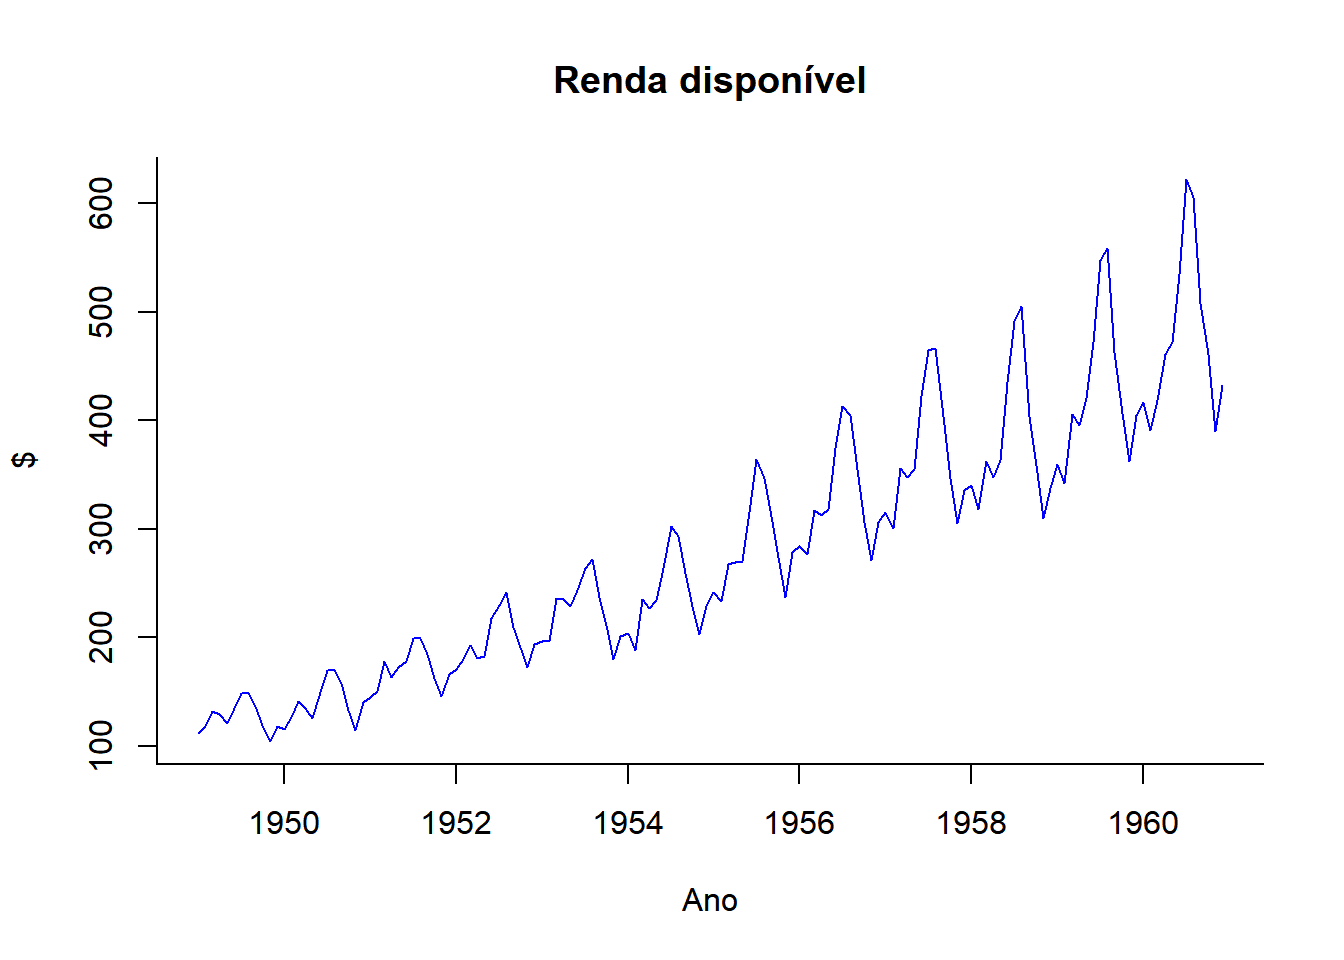
\includegraphics{Estimação-modelo-Arima_files/figure-latex/unnamed-chunk-18-1.pdf}


\end{document}
